The concept of (classical) \emph{error-correcting codes} (ECC) was
introduced by Claude Shannon in 1948 \cite{shannon}.
Fundamentally, an ECC encodes $logical$ information within
a large superset of basic information carriers.

In the case of a classical computer, this means encoding a
bitstring within a system containing more physical bits
than the length of the encoded message, with the goal of message transmission
being resilient to some bits being faulty or subject to interference (i.e. EM-interference).
Analogously, in the case of a quantum computer this means encoding a \emph{logical}
qubit within a system of multiple qubits, with a similar goal of resilience towards
errors caused by external influences.

In this chapter, we will give an overview of different quantum error correction codes,
starting with adaptations of classical codes.
\subsection{Classical codes}
The concept of (classical) error-correcting codes (ECC) was
introduced by Claude Shannon in 1948.
Fundamentally, an ECC encodes $logical$ information within
a large superset of basic information carriers.
In the case of a classical computer, this means encoding a
bitstring within a system containing more physical bits
than the length of the encoded message, with the goal of message transmission
being resilient to some bits being faulty or subject to interference (i.e. EM-interference).

Two such classical ECCs are the repetition and the ring code.
We call these codes linear because their graph representations are
linear, or one-dimensional. In Quantum error correction, we speak of $[[n,k,d]]$ stabilizer
codes if an encoding scheme allows for $n$ physical qubits to 
encode $k$ logical qubits to an error distance of $d$, i.e. $d$ 
arbitrary individual errors being corrigible.
In the following, I will refer to linear or classical codes as having a 
distance of $\frac{1}{2}$, to indicate that they do not protect against an
arbitrary single-qubit error, but only against flips in one specific eigenbasis.
\subsubsection{Repetition code}
For this error code information is encoded by repeating the 
intended message some amount of times, and then decoding it
by performing a majority vote on the transmitted message.


\begin{figure}[h!]
	\begin{center}
	\captionsetup{justification=centering,margin=2cm}
	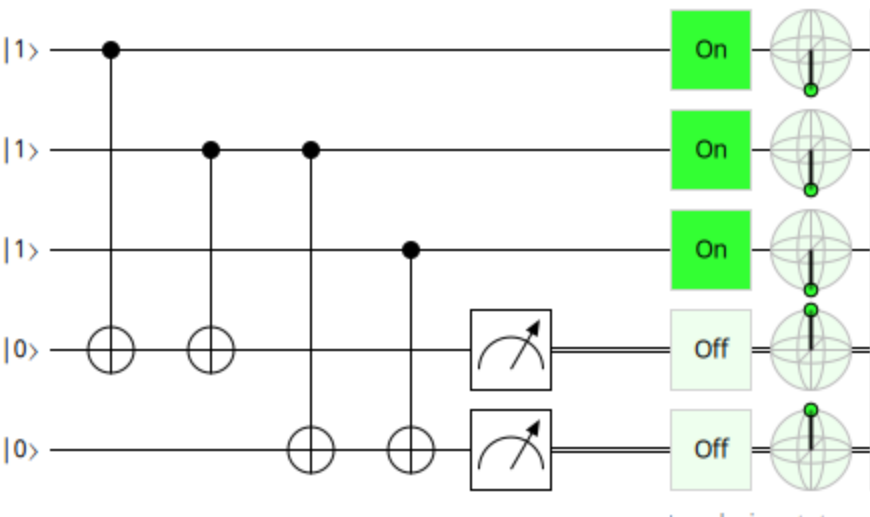
\includegraphics[scale=0.2]{./img/figures/bitflipSyndromeExtraction3Rep.png}\\
	\caption{Bitflip Syndrome extractor for [[3,1,$\frac{1}{2}$]] repetition code\\
        +1 measurement result on first ancilla indicates a bitflip error
        on qubits 1 or 2, +1 result on second ancilla indicates 
		bitflip on second or third qubit}
	\label{fig: syndrome extractor}
	\end{center}
\end{figure}

A quantum equivalent of the 3-bit repetition code performed on
the message $|1\rangle$ is the [[3,1,$\frac{1}{2}$]] repetition
code depicted in 
figure~\ref{fig: syndrome extractor}
, including so-called
$syndrome\ extraction$. A syndrome is a stabilizer that can be
measured to detect whether and where an error has occurred
in a multi-qubit system. It is crucial that the 
measurement of such syndromes occurs without harming the actual
quantum information stored in the $data-qubits$. Therefore
two additional $ancilla-qubits$ (both initialized to 
$|0\rangle$) are attached to the circuit via CNOTs.
This circuit is stabilized by IZZ and ZZI, measured by ancilla 
1/2. The measurement result will therefore be a vector of length
two, with each entry either being +1 or -1. To simplify the 
algebra this will be changed to the binary representation of 0 
for +1 and 1 for -1. 

To represent the code, Stabilizers can be stacked together to
a so-called parity-check-matrix, which satisfies:
\begin{equation}
	M_{pc}\cdot \vec{v}_{error} = \vec{v}_{syndrome}
\end{equation}
So e.g. the parity check matrix for the $[3,1,\frac{1}{2}]$
repetition code would be:

\begin{equation}
	M_{pc3} = \left( 
	\begin{array}{ccc}
		1 & 1 & 0 \\
		0 & 1 & 1
	\end{array}
	\right)
\end{equation}
And the syndrome for an X error on the first qubit would be
$\left(\begin{array}{c}1\\0\end{array}\right)$.

If we draw a graph to represent this code, with here nodes being ancillas
and edges being data qubits, we obtain the following:

\begin{figure}[h!]
	\begin{center}
	\captionsetup{justification=centering,margin=2cm}
	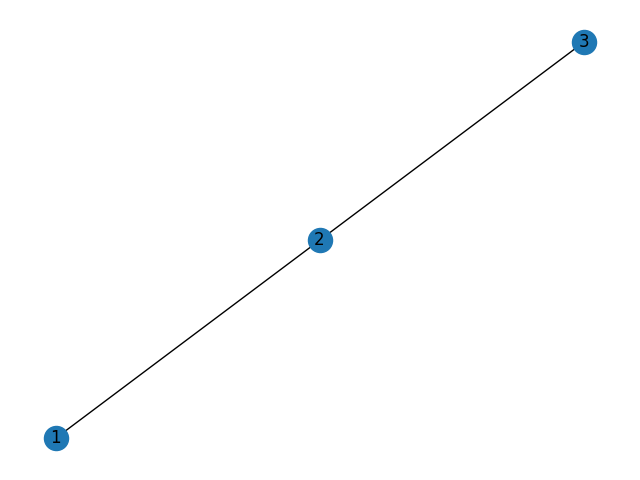
\includegraphics[scale=0.4]{./img/figures/rep_3_graph.png}\\
	\caption{Graph for [[3,1,$\frac{1}{2}$]] repetition code}
        
	\label{fig: rep_graph}
	\end{center}
\end{figure}

\newpage
\subsubsection{Ringcode}
The ring code's graph essentially just loops around at the repetition
code's single-edged ancilla nodes, so for example its edge matrix where the nth row
represents which data qubit is connected to the nth ancilla
qubit.
This matrix for a three-qubit system looks like:
\begin{equation}
    M_{pc3} = \left(
        \begin{array}{ccc}
            1 & 1 & 0\\
            0 & 1 & 1\\
            1 & 0 & 1\\
        \end{array}
        \right)
\end{equation}

\begin{figure}[h!]
	\begin{center}
	\captionsetup{justification=centering,margin=2cm}
	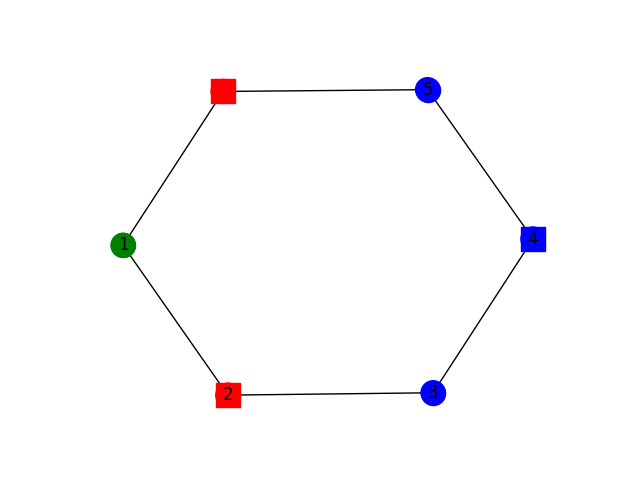
\includegraphics[scale=0.4]{./img/figures/ring_3_graph.png}\\
	\caption{Graph for [[3,1,$\frac{1}{2}$]] ring code}
        
	\label{fig: ring_graph}
	\end{center}
\end{figure}

\newpage
\subsection{Quantum Error Model}
This way of encoding information however leaves a notable
issue:

It only detects bitflip, or Pauli-X, errors occurring on
the stored quantum information. While using Hadamard gates one
could trivially adapt this code to instead detect Pauli-Z errors,
it is not possible to use linear codes like the repetition code
to $simultaneously$ detect Pauli-X and Pauli-Z errors occurring.

Unlike classical computers, on a quantum computer the type of error
 is not limited
to a bitflip. Even single qubit states have an
infinite amount of differing states to it, since when representing a single
qubit state as a vector on a Bloch sphere it immediately becomes apparent
that there are an infinite number of vectors on that sphere which are different
from it. It turns out though, that the change in state from one normalized
one to another is merely a sum of two rotations.

Fortunately, noise can therefore be modeled as a sum of Pauli gates.
Any single qubit error operator matrix E can be written as:
\begin{equation}
    E =
    \left(
    \begin{array}{cc}
        a & b \\
        c & d \\
    \end{array}
    \right) = 
    \alpha \mathbb{I} + \beta X + \delta Y + \gamma Z
\end{equation}
With an apropriate choice of $\alpha, \beta, \gamma, \delta$.
In effect, this means that with probability $\alpha$, the effect of the
error $E|\psi\rangle$ will be $\mathbb{I}$; with probability $\beta$ its effect
will be X, and so on.

It is hence sufficient to determine which of these errors $\mathbb{I}$, 
X, Y or Z has occurred, and we can apply the same operator again to return to the 
initial state.
Since an identity noise occurring is irrelevant to us, and XY as
well as ZY (anti-) commute, we need only detect for X and Z
errors occurring in order to detect any single qubit errors. 
\subsection{2D codes}
Previous research in computer science 
provides a toolset for generating valid codes
from existing encoding schemes. 
Hypergraph product codes, introduced by Tillich and Z\'emor,
of two 
existing codes will always remain a valid detection code.

The parity check matrix $H$ of a hypergraph product code is generated
by the parity check matrices of two valid codes in the following
% way:
% \begin{equation}
% 	H = \left(\begin{array}{cc}
% 		M_{pcX} & 0 \\
% 		0 & M_{pcZ} \\
% 	\end{array}\right)
% \end{equation}

\subsubsection{Surface code}
We can therefore form a hypergraph product code of two repetition
codes to
obtain the [[$d^2$,1,d]] ``Surface-Code'' which can detect up
to d of $both$ X and Z errors, and 
therefore any error happening \cite{joschka}.
We can draw this code as a graph, whereby the code's stabilizers
are understood as an adjacency Matrix of data to ancilla qubits.
Like the repetition code, the Surface code is a code that is regular until
its boundary nodes. 
The logical operators on the surface code are lines that go from one 
boundary to another that lies across, as this triggers every ancilla along
the way twice, thus nonce, and therefore takes the message back to the
codespace.

\begin{figure}[h!]
	\begin{center}
	\captionsetup{justification=centering,margin=2cm}
	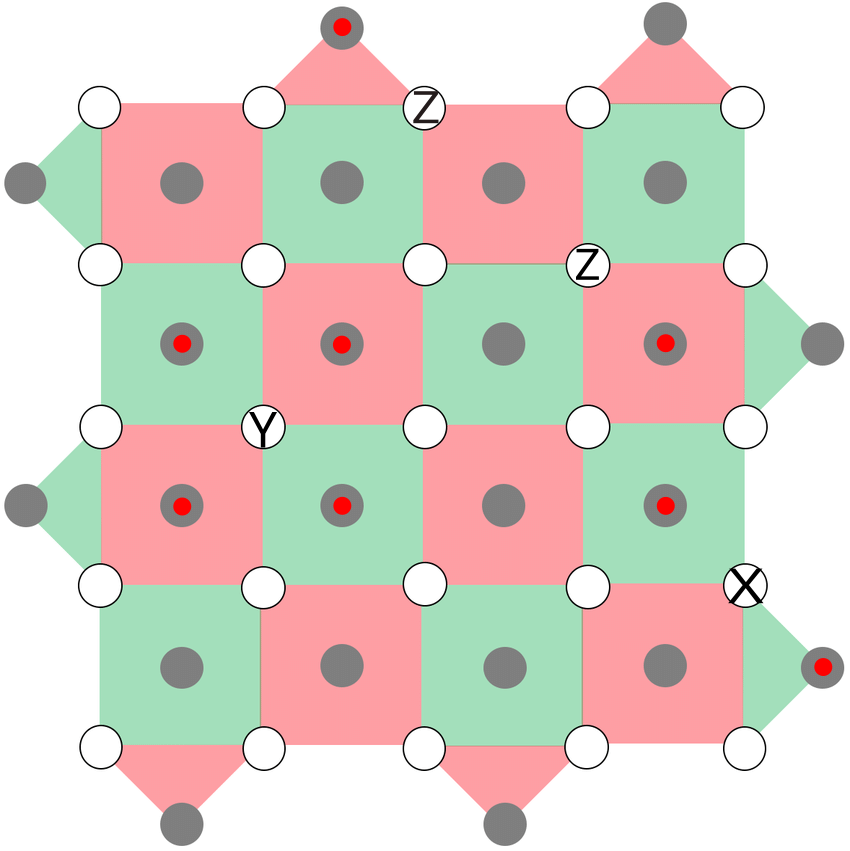
\includegraphics[scale=0.35]{./img/figures/d5surfaceCode.png}\\
	\caption{Distance 5 Surface code with data qubits in white and 
    ancilla qubits in grey. Green Faces represent Z stabilizers
    and Red faces represent X stabilizers.
    Errors on data qubits are marked
    by respective Pauli names and violated stabilizers are marked in red.}
	\label{fig: surface_code}
	\end{center}
\end{figure}


INCLUDE LOGICAL OPERATORS
\newpage

\subsubsection{Toric code}
Similarly, a hypergraph product code of two ring codes can be 
generated. We call this code the "Toric code".\\
\begin{figure}[h!]
	\begin{center}
	\captionsetup{justification=centering,margin=2cm}
	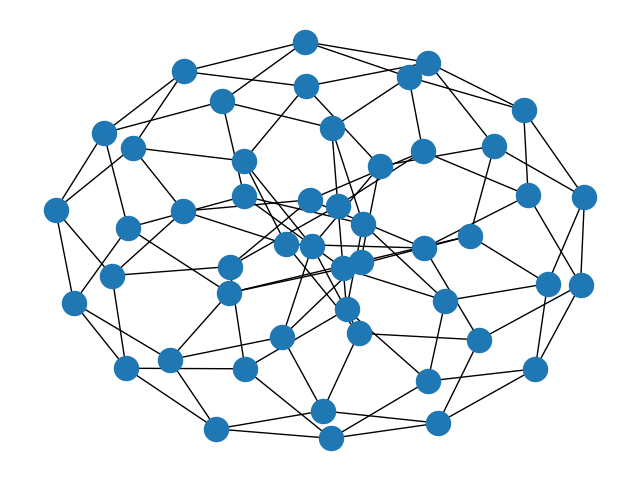
\includegraphics[scale=0.4]{./img/figures/toric_5_graph.png}\\
	\caption{Graph for [[49,1,7]] toric code}
        
	\label{fig: toric_graph}
	\end{center}
\end{figure}
Notably, this resembles a donut, or torus.
The logical operators on the toric code are loops, so a circle of 
'errors' on nodes is a logical X operator, and a circle of 'errors'
on faces is a logical Z operator.
\newpage

\subsubsection{Color code}
The color code's parity-check-matrix's 
rows are both the code's X stabilizers and Z stabilizers.
Any three-colorable and three-valent graph represents a valid color code.
On the color code, an error is bounded by syndromic faces of all colors.
The simplest color code is the [[7,1,3]] Steane code \cite{steane}. 
\\
\begin{figure}[h!]
	\begin{center}
	\captionsetup{justification=centering,margin=2cm}
	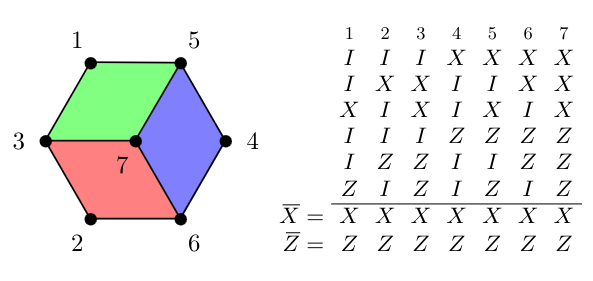
\includegraphics[scale=0.6]{./img/figures/steane.png}\\
	\caption{Graph for the [[7,1,3]] color code, also known as the
    Steane code , and its stabilizers. 
    Figure from \cite{steane}.}
        
	\label{fig: color_graph}
	\end{center}
\end{figure}
% habe ich von erster google bildsuchen seite

\newpage